\section{ADC}
\label{sec:adc}
\textit{\hyperlink{schematic.4}{schematic}}

\subsection{Overview}
\label{sec:adc-overview}

The ADC is used to digitize signals amplified by the IF \hyperref[sec:ada4940-2]{ADA4940-2}
differential amplifiers before sending them to the \hyperref[sec:xc7a15t-ftg256]{FPGA} for
processing.

\subsection{LTC2292}
\label{sec:ltc2292}

\subsubsection{Description}
\label{sec:ltc2292-description}

The LTC2292 is a 40MHz, 12-bit differential input ADC\@. This sets the Nyquist frequency at
$20 \si{MHz}$, well above the several hundred $\si{kHz}$ that characterize our signal
frequencies. By oversampling, we're able to relax anti-aliasing filter requirements, which improves
bandwidth and resolution.

\subsubsection{Pinout}
\label{sec:ltc2292-pinout}

\label{tab:ltc2292-pinout}
\begin{tabularx}{\textwidth}{>{\hsize=.2\hsize}X >{\hsize=.3\hsize}X X}
        \caption{LTC2292 pinout.} \\
        \toprule
        \# & Pin & Description \\
        \midrule

        1--2, 15--16       & AINA+, AINA-, AINB-, AINB+ & The differential inputs for channels A and
        B. The input filters are explained in \cref{sec:ltc2292-component-selection}.           \\
        3--6, 11--14       & REFHA, REFLA, REFLB, REFHB & These are the high and low reference for
        channels A and B, respectively. Their connection is specified exactly by the datasheet. \\
        7, 10, 18, 63      & VDD                        & 3.0V power supply.                    \\
        8, 9, 21           & CLKA, CLKB, MUX            & 40MHz clock inputs for channels A and B. Connecting the clock
        pins together with MUX multiplexes channels A and B together and causes the multiplexed
        output to be available on buses A and B. Fig.~\ref{fig:ltc2292-multiplex} shows the timing
        diagram for the multiplexed output. Since we only need one set of the identical signals, bus
        B is left floating.                                                                    \\
        17, 64, 65, 31, 50 & GND, OGND                  & ADC, output and power grounds are all
        connected to the same ground plane.                                                    \\
        39, 42             & OVDD                       & Power supply for the output drivers. \\
        43--48, 51--56     & DA0--DA11                  & Digitized 12-bit output data.        \\
        57                 & OFA                        & Driven high when overflow or underflow
        occurs. This is fed to the FPGA to allow overflow/underflow detection.                 \\
        26--30, 33--39     & DB0--DB11                  & The channel B data bus. Left floating (see
        description for CLKA, CLKB, MUX).                                                      \\
        40                 & OFB                        & Similar to OFA, but for channel B. Also
        exported to the FPGA\@.                                                                \\
        61, 20             & VCMA, VCMB                 & Exports a 1.5V signal to the IF differential amplifiers, which use it
        to set their common mode voltage. The $2.2 \si{\mu F}$ capacitors are specified by the
        datasheet.                                                                             \\
        24--25, 41--42     & NC                         & No connect.                          \\
        59, 22, 58, 23     & SHDNA, SHDNB, OEA, OEB     & Allow the FPGA to control the ADC's
        operation. Pulling SHDNA and OEA low operates channel A normally, while bringing them both
        high puts channel A in sleep mode. Channel B works the same way.                       \\
        62, 19             & SENSEA, SENSEB             & Tied to VDD, which specifies that the input voltage range of the
        differential signals for channels A and B is $1.5 \si{V} \pm 1
        \si{V}$ (i.e. 1.5V common-mode voltage with a 2V range).                               \\
        60                 & MODE                       & Tied to VDD, which specifies the output
        format as 2s complement and turns off the clock duty stabilizer, which should be unnecessary
        because the input clock has a 50\% duty cycle.                                         \\

        \bottomrule
\end{tabularx}

\begin{figure}[h]
        \centering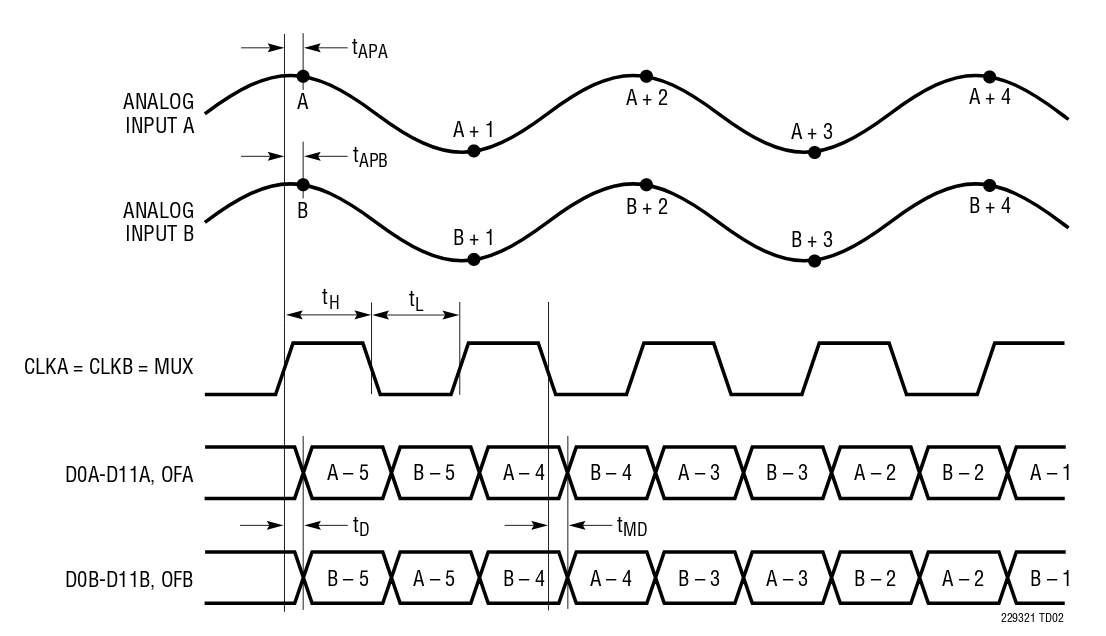
\includegraphics[width=0.75\textwidth]{data/LTC2292-multiplex.png}
        \caption{Multiplexed digital output bus timing for the LTC2292 ADC.}
        \label{fig:ltc2292-multiplex}
\end{figure}

\subsubsection{Component Selection}
\label{sec:ltc2292-component-selection}

The analog inputs employ anti-aliasing filters. The filters provide several benefits: (1) they
reduce aliasing by attenuating signals above the Nyquist frequency, (2) they limit wideband noise at
the input at the ADC input, which is important because the converter has a $575 \si{MHz}$ full-power
bandwidth, and (3) they isolate the \hyperref[sec:ada4940-2]{IF amplifier} from ADC noise at the
sampling frequency. Lastly, the capacitors act as a necessary charge source for the ADC input
capacitor. The two outer $100 \si{pF}$ capacitors (between the signal lines and ground) provide CMR
low-pass filtering with a cutoff frequency of $32 \si{MHz}$ (equation given in
Eq.~\ref{eq:anti-alias-cm-lp-filter}). The capacitor between the signal lines provides differential
low-pass filtering with a cutoff frequency of $16 \si{MHz}$. A
\href{https://e2e.ti.com/blogs_/archives/b/precisionhub/archive/2015/11/06/three-guidelines-for-designing-anti-aliasing-filters}{post
  from TI} explains this filtering. It's also important to keep the series resistor value low, since
the greater the resistance, the greater the Johnson noise.

\begin{equation}
        \label{eq:anti-alias-cm-lp-filter}
        f_{\text{c}} = \frac{1}{2 \pi R C}
\end{equation}

\subsubsection{PCB Layout}
\label{sec:ltc2292-pcb}

The $100 \si{nF}$ capacitors connected between the REFxx pins should placed as close to the pins as
possible.

The differential input traces should run parallel to one another and should be placed close
together. Additionally, they should be made as short as possible.

%%% Local Variables:
%%% mode: latex
%%% TeX-master: "fmcw-radar"
%%% End:
